\documentclass{standalone}
\usepackage{pgfplots}
\pgfplotsset{compat=1.17}
\begin{document}
% Basit 2D grafik
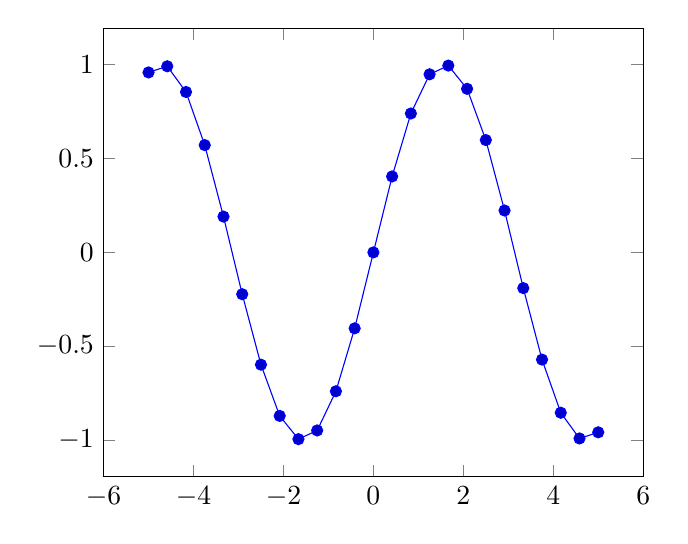
\begin{tikzpicture}
\begin{axis}
\addplot {sin(deg(x))};
\end{axis}
\end{tikzpicture}

% Başlık, eksen ve gridli grafik
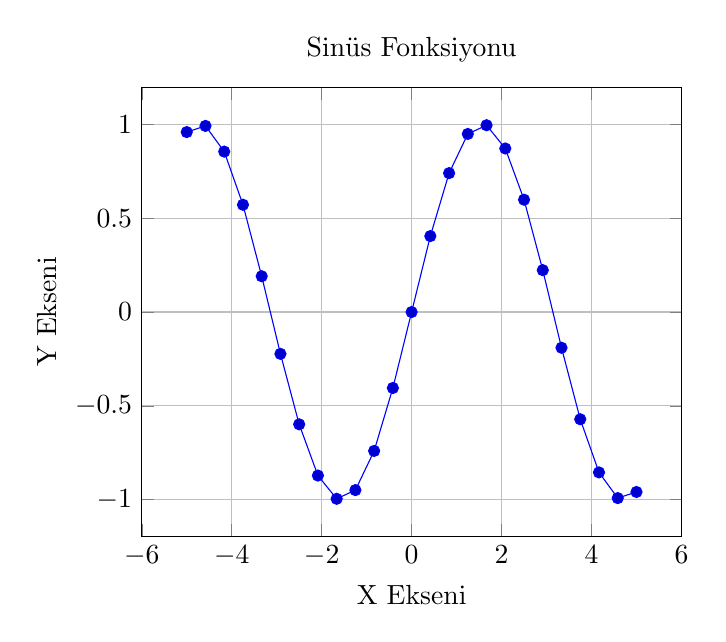
\begin{tikzpicture}
\begin{axis}[
    title={Sinüs Fonksiyonu},
    xlabel={X Ekseni},
    ylabel={Y Ekseni},
    grid=major
]
\addplot {sin(deg(x))};
\end{axis}
\end{tikzpicture}

% 3D yüzey grafiği
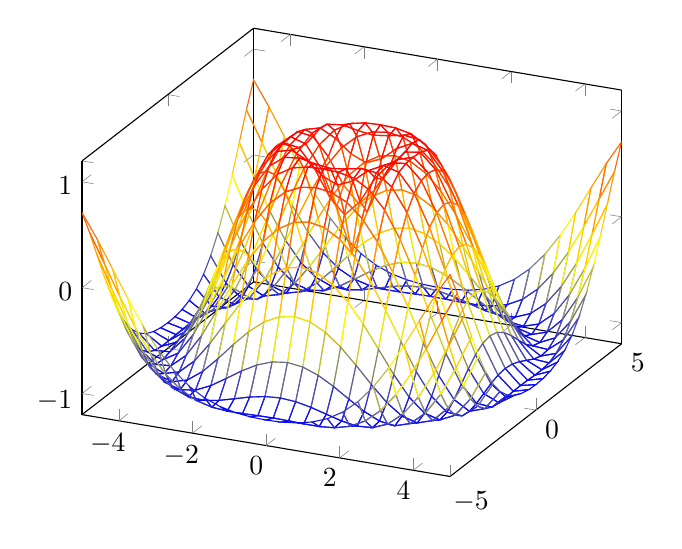
\begin{tikzpicture}
\begin{axis}
\addplot3[
    surf,
    mesh,
    domain=-5:5,
    domain y=-5:5,
    samples=25,
    samples y=25
]
{sin(deg(sqrt(x^2 + y^2)))};
\end{axis}
\end{tikzpicture}
\end{document}
